\chapter{Localization funnels, repository indexes, and freshness checks}
\label{ch12-localization-funnels-repository-indexes-freshness-checks}
\begin{quote}
\textbf{Evidence profile.} 6 strong · 5 directional · 0 corroborating evidence items across 3 developed practices (ERCA-078, ERCA-084, ERCA-174).

\textbf{Chapter claim.} Evidence without revision identity is stale, not current.
\end{quote}

In one evaluation of my memory system, run across four seeds, the task required passing a recalled value exactly as a tool argument. Retrieval by stable memory identity scored 1.0. Retrieval by token similarity returned superseded values and scored 0.0.

The similarity lane had not malfunctioned. It returned real, highly ranked records that described a state the system had already left behind. This author-system case carries no evidentiary weight, but it separates two questions that a retrieval score can collapse into one: whether a result ranks well, and whether it still describes the repository or system the worker is acting on.

Repository work presents three related architectural decisions. Some tasks benefit from a funnel that separates coarse file selection from fine edit selection. Some require typed structural relationships because the issue language and the change site share no useful vocabulary. Every retriever, index, and cache also describes a particular repository state, which may expire while its answers remain fluent and specific.

Each decision carries a different cost. A funnel adds handoffs, and an early omission propagates through every later stage. A typed index requires construction, language coverage, storage, query tools, and continuing maintenance. A freshness gate can reject useful evidence when its identity checks are too coarse. I therefore treat all three as architecture choices with observable failure modes rather than as retrieval features to add by default.

\hypertarget{stage-localization-before-repair}{%
\section{Stage localization before repair}\label{stage-localization-before-repair}}

Hierarchical localization determines where each comparison occurs and what evidence crosses the boundary between stages. Xia et al.~(\href{https://arxiv.org/abs/2407.01489}{2024}) removed open-ended tool-use autonomy from repository repair and retained three fixed phases: hierarchical localization, repair, and patch validation. On SWE-bench Lite, a curated subset of SWE-bench, that pipeline outperformed the autonomous agents evaluated alongside it while costing substantially less.

Each phase received bounded input, produced a bounded artifact, and handed that artifact to the next phase. The result showed that staged narrowing could recover much of the value then attributed to open-ended agency. Later systems built on stronger models moved ahead of that fixed pipeline, which limits the conclusion. The transferable design principle is to separate narrowing decisions and validate the transition between them; neither the original pipeline nor a general claim against agency follows from the result.

Repository structure may identify the correct region without identifying the function or statement that owns a failure. In a disconnect case, search may return a response writer, several transport adapters, and a lifecycle callback. The state transition responsible for the malformed response may sit behind that callback in another package.

The evidence needed to select the package differs from the evidence needed to select the function and edit location. A localization funnel separates those comparisons:

\begin{verbatim}
repository structure
    -> candidate files
        -> candidate symbols
            -> concrete edit locations
                -> patch validation
\end{verbatim}

Each stage should reduce the candidate set and leave an inspectable handoff.

In the disconnect case, the first stage narrows the repository to the transport and lifecycle packages. The file handoff retains the response writer and callback and records why each survived. Symbol inspection follows the callback to the function that changes response state. The final stage proposes a guard at that assignment, and validation exercises the disconnect path. If an intermediate check shows that the state owner was omitted, the funnel widens before repair begins.

The stages have asymmetric consequences. Validation can sometimes correct a mistaken edit location after a patch fails. A file omitted during the first stage is unavailable to every later stage, however capable the repair model may be. The maximum recall of the complete pipeline is therefore capped by file selection.

\begin{figure}[htbp]
\centering
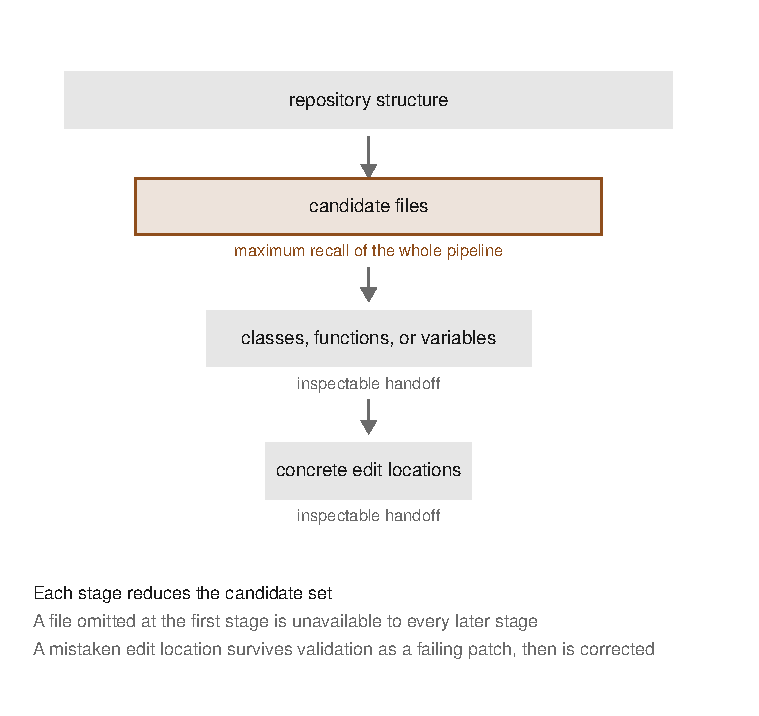
\includegraphics{figures/ch12-localization-funnel.pdf}
\caption{The localization funnel progressively narrows repository evidence, while candidate file selection caps recall because any omitted file remains unavailable to every later inspection and edit stage.}
\end{figure}

Inspectable handoffs make downstream errors visible, but validation can repair a poor edit choice only when the necessary file survived initial selection.

Sepidband et al.~(\href{https://arxiv.org/abs/2604.05481}{2026}) measured this asymmetry across 500 SWE-bench Verified instances and 61 context configurations. Relative to the no-file condition, adding file-level context produced 15 to 17 times as much repair improvement as later localization refinements.

The same experiment found that successful repairs clustered around approximately six to ten relevant files for the model family studied. That range is useful as a diagnostic band, not as a quota for other models, repositories, or task distributions. Both findings come from one benchmark and one sweep of context configurations.

The practical implication is to measure file selection before adding more reasoning downstream. Chapter 11's decomposed scoring makes that diagnosis possible. When file \(\mathrm{Recall}@k\) is low, a stronger patch generator is being evaluated on a candidate set that often excludes the answer. When file recall is already high and repair still fails, additional localization machinery may move cost into a stage that is no longer limiting the system.

\Needspace{5\baselineskip}

The funnel also constrains what context should cross each boundary. A file-selection stage should not silently pass its complete search transcript downstream, because doing so recreates the mixed-granularity problem inside a larger prompt. Its handoff should identify:

\begin{itemize}
\tightlist
\item
  the files retained;
\item
  the evidence for retaining them;
\item
  the candidates rejected; and
\item
  any uncertainty that remains.
\end{itemize}

The next stage can then inspect those files for structural candidates without inheriting every abandoned hypothesis.

Inspectable handoffs also create validation points. Before symbol inspection begins, a file set can be checked against import neighborhoods, ownership boundaries, or another retrieval lane. Before concrete lines are proposed, the symbol set can be checked for definitions, references, and state ownership. These checks need not be performed by an autonomous agent. They need only expose a miss while widening remains possible.

Skipping a stage may appear cheaper because it removes a model call or retrieval pass. Xia et al.~reported the opposite. When their pipeline moved directly from file selection to edit locations, both cost and performance worsened because the remaining stage had to search too much source at once. Removing a stage increased the work inside the stage that remained. Pipeline length is therefore a poor proxy for pipeline cost.

Chang et al.~(\href{https://arxiv.org/abs/2502.15292}{2025}) trained separate models for file, function, and statement localization and found value in treating each level as a distinct representation and discrimination problem. That support is directional and does not determine the implementation. A fixed prompt, cheap classifier, retrieval operation, or stronger general model may be appropriate at a particular stage depending on workload, accuracy, and latency.

The funnel fits issue-resolution work because those tasks often decompose into localization, repair, and validation. It is less convincing for exploratory refactoring, architecture discovery, or changes whose scope becomes visible only after editing begins. Those workloads require an explicit return path that can widen the candidate set after a failed hypothesis. Without one, a rigid pipeline continues refining the wrong corpus.

Later agent systems that surpassed the fixed pipeline also limit any claim that autonomy itself was unnecessary. Stronger models can search, revise, and use tools while preserving hierarchical localization. The evidence supports measuring the fixed narrowing architecture first and then asking which remaining failures autonomy repairs. It does not support freezing the pipeline around one generation of models.

The companion material covers narrower implementation choices: structural retrieval as a lane beside text search, stable structural anchors injected into context, and query-time graph walks when stored expansion would become too large. Those choices follow the architectural decision developed here. Preserve granularity, validate each handoff, and measure file selection as the stage capable of foreclosing every later success.

\hypertarget{build-a-typed-index-only-when-someone-will-maintain-it}{%
\section{Build a typed index only when someone will maintain it}\label{build-a-typed-index-only-when-someone-will-maintain-it}}

Consider an issue reporting that cancelling one export leaves later exports blocked. The change belongs in a generic state-transition helper reached through a queue consumer and shared lifecycle component. None of those artifacts uses the language of exports or cancellation.

Exact search can find the user-facing entry point. Similarity search can find code that resembles the reported symptom. Neither query expresses the dependency path from the entry point to the component that owns the blocked state. A typed index can answer that path question, but the decision to build one begins with maintenance. If no named owner accepts the continuing work, the projected retrieval gain has no durable system behind it.

\Needspace{5\baselineskip}

That work includes:

\begin{itemize}
\tightlist
\item
  parsing each supported language;
\item
  assigning stable identities to entities;
\item
  recording typed relationships;
\item
  handling generated code and partial parses;
\item
  publishing updates without exposing incomplete state;
\item
  versioning the schema and query surface; and
\item
  testing correspondence between index results and repository state.
\end{itemize}

Each new language or artifact type extends the obligation. Index construction is a continuing product surface even when users encounter it only through search results.

The cheaper alternative is often a generated repository map or skeleton placed near the front of the model's context. It can list directories, important files, top-level symbols, and ownership boundaries. Navigation then relies on inexpensive operations such as exact search, opening definitions, finding references, and listing callers.

A repository map cannot answer arbitrary multi-hop questions. It is, however, easy to regenerate and inspect. For a modest repository, low change rate, or occasional task, that trade may be preferable to maintaining a graph service.

A typed index becomes plausible when the workload repeatedly asks structural questions that the map cannot express. The representation parses directories, files, classes, functions, and linked development artifacts into typed nodes. In the export example, invocation and reference edges connect the queue consumer to the lifecycle component and then to the state helper. A broader index may also record containment, imports, inheritance, definitions, ownership, and links to issues or tests.

This representation is a \textbf{typed knowledge graph}. It stores entities under declared kinds and records how each pair of connected entities relates. The types constrain traversal and make a returned path inspectable. They also create schema, parser, identity, and migration obligations that a similarity index does not have.

The export question can then become a bounded traversal:

\begin{verbatim}
start: export handler named by the issue
    -> follow invocation edges into the queue consumer
    -> follow references into the lifecycle component
    -> return functions that write the blocked state
\end{verbatim}

The issue and the final helper need no shared token. The graph supplies a path that can be inspected edge by edge.

A structural path can also be more compact than the alternatives. Instead of serializing the repository or opening every file encountered during exploration, the retriever can return a small subgraph containing the entry point, intermediate calls, state owner, and relationship types. The model receives both the candidates and an explanation of why they were selected.

Published results show why teams consider paying this cost. Chen et al.~(\href{https://arxiv.org/abs/2503.09089}{2025}) reported 92.7 percent file-level localization accuracy for LocAgent, with performance declining at finer granularities. That pattern supports using the graph to protect file localization while measuring symbol and line localization separately. The figure describes localization, not repair, and should not be read as an issue-resolution rate.

LocAgent's fine-tuned 7B and 32B models approached the reported Claude 3.5 localization accuracy at approximately 86 percent lower cost. Its ablations also showed that the gain depended on the complete search and traversal toolset around the graph, not on the stored representation alone.

Yang et al.~(\href{https://arxiv.org/abs/2503.21710v1}{2025}) provide more direct but weaker evidence for multi-hop demand. Among bugs their repository-aware graph successfully localized, 69.7 percent required traversal across several relationships. That figure comes from the first paper revision, and headline results changed later. It also comes from SWE-bench Lite. The result establishes direction within one benchmark, not the prevalence of multi-hop demand in an arbitrary production repository.

The same study capped repair input at the top 20 functions. That cap is part of the architecture. A traversal system can continue finding plausible neighbors after useful evidence has been exhausted. Passing every discovered node to the generator allows additional candidates to interfere with repair. A graph can therefore improve localization while degrading generation when no boundary separates the two stages.

Ma et al.~(\href{https://arxiv.org/abs/2406.01422}{2024}) measured this tension in LingmaAgent across a larger exploration budget. Its issue-resolution rate rose from 16.0 percent with no exploration iterations to 21.3 percent at 600 iterations. Exploration continued to uncover useful code across that range.

The patch-application rate, which measured whether generated diffs applied cleanly, peaked at 200 iterations and then declined through 600. Clean application was necessary but not sufficient for resolution. Fewer patches could apply while more tasks were resolved if the patches that did apply were more often correct. The result suggests that additional exploration continued to improve localization while making the downstream generation problem harder.

Both measurements come from one benchmark configuration. The paper reports the 200-iteration location of the application-rate peak but not the curve's values, so the peak is useful only as a prompt to measure the local stopping point.

A traversal budget must therefore be evaluated against both localization and patch application. It may stop after a fixed number of expansions, when no new relationship type appears, or when the candidate set reaches the repair budget. The literature does not identify one stopping rule that dominates across repositories.

\Needspace{5\baselineskip}

A defensible local rule requires recording:

\begin{itemize}
\tightlist
\item
  each expansion;
\item
  the relationship followed;
\item
  candidates admitted and pruned;
\item
  the downstream candidate limit; and
\item
  the point at which further exploration stopped changing repair outcomes.
\end{itemize}

On SWE-bench Lite, the same study reported an 18.5 percent relative improvement over SWE-agent. That result applies to the benchmark configuration. Its production report used different operating measures: 16.9 percent of in-house issues were resolved automatically and 43.3 percent after human intervention. Automatic resolution, assisted resolution, and benchmark performance describe different systems and should not be combined.

Two additional experiments extend the evidence without removing its limits. Ouyang et al.~(\href{https://arxiv.org/abs/2410.14684}{2024}) added RepoGraph, a line-level definition and reference graph, as a plug-in and reported gains in both pipeline-style and agent-style frameworks. CodexGraph, from Liu et al.~(\href{https://arxiv.org/abs/2408.03910}{2024}), provides directional support for graph queries when similarity retrieval has weak multi-hop recall. Together they support a specialist structural lane that can attach to different orchestration styles.

Fine-grained localization remains difficult. LocAgent's accuracy declined below the file level, and serializing a graph as text can erase distinctions explicit in storage. Edge direction, relationship type, entity scope, and alternative paths can collapse into an ordering the model misreads. Extending the graph below functions may help line-level work, but it also increases node count, serialization cost, and the number of nearly equivalent candidates.

Query construction adds another failure surface. A valid graph can return an irrelevant answer because the model selected the wrong starting entity, followed the wrong relationship, or stopped one hop too early. Bounded operations such as \texttt{find\ definitions}, \texttt{list\ callers}, and \texttt{follow\ imports} are easier to validate than a general graph query generated in one attempt. Simple entity questions should use those cheaper operations, reserving the graph for structural questions that require it.

The representation returned to the model must also be measured. An index may emit paths, source excerpts, signatures, summaries, edge lists, or a combination. Each format changes token cost and the evidence available to the generator. A compact summary may omit the exact call that proves relevance. Raw source may conceal the path that made it relevant. Serialization is therefore part of the retrieval design rather than a presentation detail.

My architecture-analysis toolkit provides one author-system example. Its typed symbol graph measures change propagation by counting files reachable from a changed entity within a bounded depth. The same representation can support impact analysis through relationships that lexical similarity does not encode. This is narrative corroboration and supplies no evidence about agent repair rates.

The index owner must also own correspondence with the repository. Incremental parsers fail, branches diverge, generated artifacts retain obsolete identities, and linked issue data changes independently of code. An index that is not checked against repository state after those events silently answers questions about an earlier repository.

\Needspace{5\baselineskip}

Every returned path should therefore carry enough identity to establish:

\begin{itemize}
\tightlist
\item
  the repository and branch;
\item
  the source revision;
\item
  the index and schema versions;
\item
  the entity identities;
\item
  the freshness status; and
\item
  any parse or ingestion failures affecting the path.
\end{itemize}

Readers unwilling to fund that admission and maintenance path should choose a generated repository map and fixed navigation operations explicitly. Readers willing to fund it should cap candidate sets, budget traversal, validate query construction, test serialization, and measure the graph as one component of the surrounding retrieval system.

The maintenance cost is justified only while a named owner can show which repository state each answer describes.

\hypertarget{admit-only-evidence-tied-to-the-current-state}{%
\section{Admit only evidence tied to the current state}\label{admit-only-evidence-tied-to-the-current-state}}

Weng et al.~(\href{https://arxiv.org/abs/2605.14478}{2026}) changed Python helper signatures in 17 curated examples and compared stale with current retrieved snippets. This small diagnostic study is the only literature support for the practice developed here. It establishes the direction of the failure, but one form of staleness tested on two models supplies neither a general effect size nor a safe refresh cadence.

Under stale-only retrieval, Qwen2.5-Coder-7B-Instruct produced 15 outputs incompatible with the current helper signature, and gpt-4.1-mini produced 13. Both models received the same 17 examples. Under current-only retrieval, neither produced an incompatible output.

These paired results support a narrow architectural rule: retrieved code should enter model context only when the system can tie it to the repository state the worker is allowed to modify.

A stale result is an active hazard rather than an ordinary retrieval miss. It offers a concrete and plausible description of an API that no longer exists. High rank cannot compensate for evidence drawn from the wrong state.

The contrast with no retrieval makes the failure sharper. Without retrieved context, the models tended to fail without calling the obsolete signature. With stale context, they generated executable-looking code against the wrong contract. Retrieval converted uncertainty into a specific but incompatible implementation.

Adding current evidence reduced that harm even when stale snippets remained present. Across the tested model and retrieval conditions, adding valid current snippets to stale ones lowered the rate of current-state-incompatible outputs by 47 to 65 percentage points relative to stale-only retrieval over the same 17 examples. Permuting result order produced no significant difference. In this diagnostic, the presence of current evidence mattered more than whether it appeared first.

The paired comparison corresponds to the binary-outcome design in Chapter 1. Both conditions used the same 17 examples, each outcome was compatible or incompatible, and McNemar's test analyzed the discordant pairs.

The exact two-sided values were \(6.1 \times 10^{-5}\) for Qwen2.5-Coder-7B-Instruct and \(2.4 \times 10^{-4}\) for gpt-4.1-mini. Under the null hypothesis of no difference between retrieval conditions, each value gives the probability of observing discordance at least as extreme as the measured result.

Those values establish a difference within the curated sample. They do not estimate the effect size in another repository.

The study does not show that stale retrieval will fail at similar rates elsewhere, that every form of drift is equally harmful, or that one refresh interval is safe. Helper-signature changes are unusually direct because stale code presents a callable contract. Changes to behavior, configuration, ownership, or surrounding assumptions may fail differently and may be harder to observe.

\Needspace{5\baselineskip}

A freshness gate needs two identities:

\begin{itemize}
\tightlist
\item
  the repository state from which the retrieval artifact was built; and
\item
  the repository state the worker is allowed to edit.
\end{itemize}

A commit identity can represent a clean tree. When relevant files contain uncommitted changes, the commit alone is insufficient because it describes a state different from the worker's current view. The gate then needs content identities for the affected files or another representation of the working state.

Every retrieval response should carry its indexed state identity so the caller can compare it with the working state before exposing any snippet to the model.

The comparison belongs at the retrieval boundary. Checking only when indexing begins leaves a race in which files change during construction or after a long-running query starts. A safe builder reads from a fixed snapshot, constructs the new index privately, and atomically publishes the completed generation together with its state identity. Queries then observe one complete generation rather than a mixture of old and new records.

Suppose an index was built from a clean commit and a worker later edits a helper without committing it. A query returns the old signature together with the index commit. The gate checks the in-scope working file, detects that its content no longer matches the indexed state, and withholds the snippet before generation begins.

Live exact search can supply the current helper while the richer index rebuilds. The builder snapshots the edited state, publishes a completed generation with the new identity, and repeats the original query. The caller admits the new result only after its identity matches the worker's state.

Concurrent work makes the choice of identity important. Two agents may share a base commit while holding different uncommitted edits. A commit-level check can therefore admit evidence stale for both working trees. Hashing every file in a large repository on every query may be too expensive.

\Needspace{5\baselineskip}

A practical design can:

\begin{itemize}
\tightlist
\item
  pin the base commit;
\item
  track content identities for files covered by each response;
\item
  invalidate affected entries from filesystem events; and
\item
  reconcile periodically against the actual working tree.
\end{itemize}

The system should measure both the coverage of that check and the race window it leaves open.

Caches require the same treatment. A query cache keyed only by search text can return an obsolete result after the underlying index refreshes. Repository-state identity must participate in the cache key, or the cache entry must be invalidated when a new index generation publishes. Otherwise the freshness gate protects the index while a faster layer bypasses it.

Retries also need a state transition. If a query fails because its index generation is stale, retrying against the same generation cannot improve the result. The retry must wait for or request a generation built from an accepted state and then repeat the query against that generation.

A timeout can bound the wait, but it should end in an explicit freshness failure rather than silently returning stale evidence.

Refusal has an operational cost. Live exact search may remain current while a structural or semantic index rebuilds. The system can therefore fall back to lower-capability navigation that is tied to the working state. When no current source is available, a visible miss that preserves uncertainty is safer than a fluent answer built from an obsolete API. The generator can request more evidence or fail explicitly rather than act on a false contract.

The literature reviewed for this chapter supplies no universal refresh cadence. Repository change rate, index-build duration, query latency, and the consequence of stale evidence can inform a local policy, but they do not yield an evidence-backed interval.

\Needspace{5\baselineskip}

Event-driven refresh can shorten the stale window after ordinary edits, although missed events and parser failures still require reconciliation. Scheduled rebuilding can provide that reconciliation, but its period should follow measured drift and recovery cost. Useful retrieval metrics include:

\begin{itemize}
\tightlist
\item
  the age of admitted results;
\item
  the frequency of state mismatches;
\item
  the duration of rebuild windows;
\item
  the rate of freshness refusals; and
\item
  the success and cost of fallback navigation.
\end{itemize}

My session-snapshot system illustrates a strict version of this gate. It pins cryptographic hashes for all in-scope files together with the repository commit. Any drift marks the snapshot stale, and the system regenerates it rather than branching from it. Remotely sourced repository knowledge is excluded because the system cannot bind it to the same content check.

My published literature-review index provides the counterexample. One surface advertised a paper count that disagreed with the linked page, and synchronized copies diverged further. The index continued to appear authoritative after it stopped describing its own contents. This contrary case exposes the maintenance cost of the prescription: a freshness policy that no one operates becomes another stale artifact.

Freshness does not determine authorization. Permission policy requires separate identities, rules, and audit records. The evidence here supports refusing obsolete repository states. It does not establish who may retrieve a current one.

\hypertarget{choose-the-next-retrieval-intervention}{%
\section{Choose the next retrieval intervention}\label{choose-the-next-retrieval-intervention}}

Begin with Chapter 11's decomposed measurements and determine which stage is limiting the operated system. Inspect file-level retrieval before changing the agent architecture.

File \(\mathrm{Recall}@k\) asks whether the repair stage receives the necessary files at all. When those files rarely appear, improve file selection and staged localization before adding more open-ended reasoning. A stronger repair model cannot act on evidence the retrieval path excluded.

\Needspace{5\baselineskip}

Next, decide whether repeated structural questions justify a typed index. Before approving the build:

\begin{itemize}
\tightlist
\item
  name the owner;
\item
  define the supported languages and relationship types;
\item
  specify how repository correspondence will be maintained;
\item
  cap the candidates the index can send downstream;
\item
  define its publication and rollback process; and
\item
  record how freshness failures will be detected.
\end{itemize}

When no one owns that lifecycle, choose the cheaper architecture explicitly: a generated repository map near the front of context, together with exact search, definition lookup, reference search, and bounded caller navigation.

Every index, snapshot, and cache should carry a commit or content identity. Compare that identity with the worker's current state at retrieval time. Record mismatches as an operating metric, and refuse the result or fall back to current navigation when the identities differ.

A freshness refusal is visible and recoverable. A stale result can silently become the basis of a plausible patch.

Chapter 13 turns from which evidence the system retrieves to how much of that evidence the model can use.

\textbf{Portable claim.} Evidence without revision identity is stale, not current.

\section*{Sources and evidence}

\textbf{Stage localization before repair}

\begin{itemize}
\tightlist
\item
  Strong evidence: Xia, C. S., et al.~(2024), ``Agentless: Demystifying LLM-based Software Engineering Agents,'' arXiv:2407.01489.
\item
  Directional evidence: Chang, J., et al.~(2025), ``BugCerberus: Bridging Bug Localization and Issue Fixing,'' arXiv:2502.15292. (Per-hierarchy-level specialization.)
\item
  Strong evidence: Sepidband, M., Viet Pham, H., Hemmati, H. (2026), ``On the Role of Fault Localization Context for LLM-Based Program Repair,'' arXiv:2604.05481.
\item
  Corroboration: none on record.
\end{itemize}

\textbf{Index the repository as a knowledge graph}

\begin{itemize}
\tightlist
\item
  Strong evidence: Chen, Z., et al.~(2025), ``LocAgent: Graph-Guided LLM Agents for Code Localization,'' arXiv:2503.09089.
\item
  Directional evidence: Yang, B., et al.~(2025), ``Enhancing Repository-Level Software Repair via Repository-Aware Knowledge Graphs'' (KGCompass), arXiv:2503.21710. (The 69.7 percent multi-hop figure is carried from v1; later versions report different headline values, so the inline link pins v1.)
\item
  Strong evidence: Ma, Y., et al.~(2024), ``Alibaba LingmaAgent: Improving Automated Issue Resolution via Comprehensive Repository Exploration,'' arXiv:2406.01422.
\item
  Directional evidence: Liu, X., et al.~(2024), ``CodexGraph: Bridging Large Language Models and Code Repositories via Code Graph Databases,'' ICLR 2025, arXiv:2408.03910.
\item
  Strong evidence: Ouyang, S., et al.~(2024), ``RepoGraph: Enhancing AI Software Engineering with Repository-level Code Graph,'' arXiv:2410.14684.
\item
  Strong evidence: AOCI AI-oriented code indexing (Liu 2026), arXiv:2605.02421.
\item
  Directional evidence: MAGIS (Tao 2024), arXiv:2403.17927.
\end{itemize}

\textbf{Gate retrieval on freshness}

\begin{itemize}
\tightlist
\item
  Directional evidence: Weng, H., et al.~(2026), ``When Retrieval Hurts Code Completion: A Diagnostic Study of Stale Repository Context,'' arXiv:2605.14478.
\end{itemize}
